\section{Gripper Technologies}
\label{sec:grippers_technolgy}

End-effectors are hardware devices of handily mechanisms (e.g., robots and automation
systems) aiming them to interact with the environment.

Two classes of interaction are: passive and active.

In passive interaction, the end effectors are composed of sensors (e.g., inspection, quality assurance, and surveillance applications). Meanwhile, the active interaction consists of direct interaction with the workpiece (e.g., welding, cutting, drilling, screwing, grinding, painting, and grasping different objects).

\begin{figure}[h!]
\resizebox{0.85\textwidth}{!}{%
\begin{tcolorbox}
    \centering
    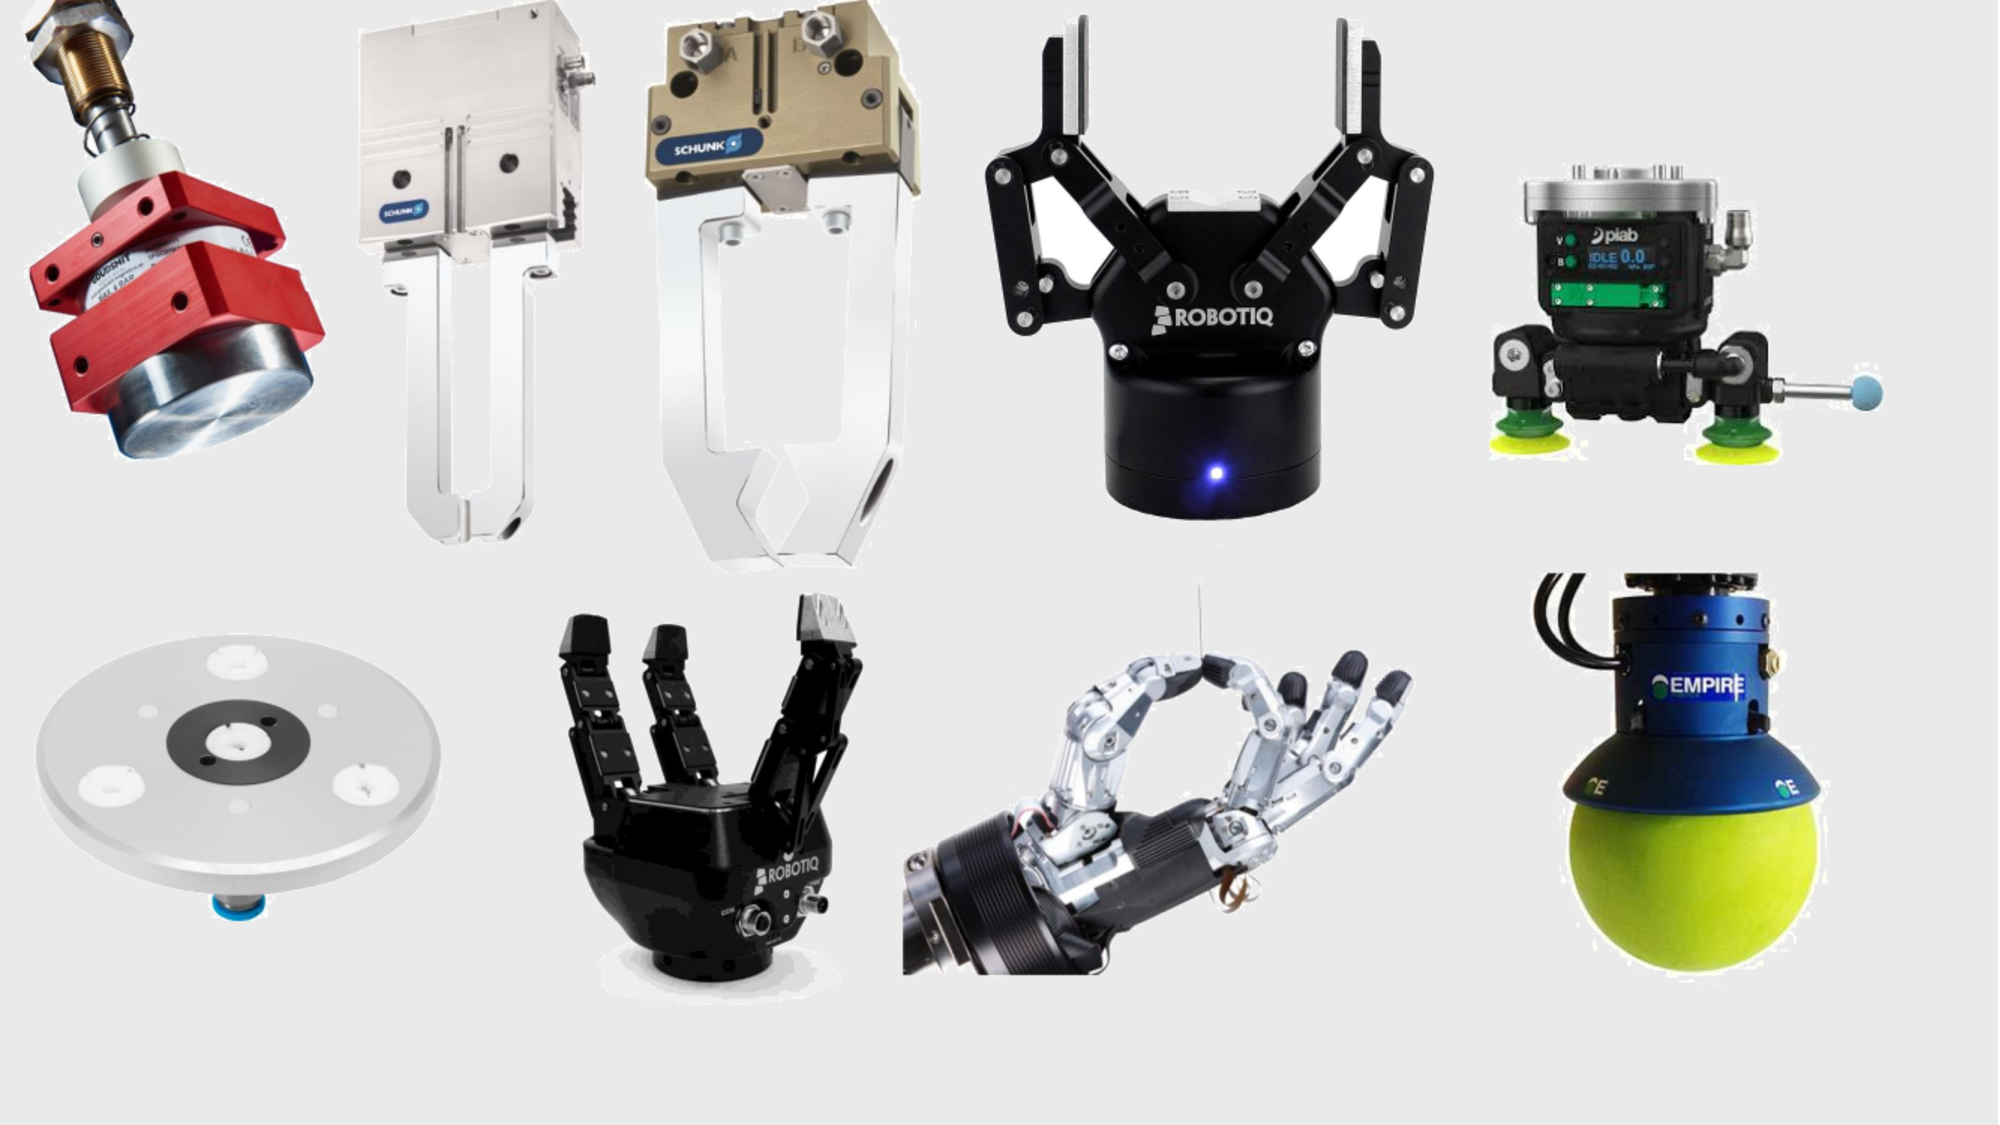
\includegraphics[trim={0mm 2cm 2cmm 0mm},clip,width=1\linewidth,angle=0]{Cap3/Figuras/grippers_list_gray_bg.pdf}
\end{tcolorbox}
    \caption{Commercial grippers examples. From top-left to down-right:  magnetic \cite{magnetic}, parallel fingers \cite{parallel}, angular fingers \cite{angular}, adaptive two-fingers \cite{robotiq_grippers}, dual suction \cite{dual_suction}, Bernoulli\cite{bernoulli}, adaptive three-fingers \cite{robotiq_grippers}, anthropomorphic \cite{anthopomorphic}, Versaball \cite{versaball}}
    \label{fig:gripper_examples}
    }%end of resize box
\end{figure}

The robotic grippers are a complex class of active end-effectors. They are active links to handle workpieces~\cite{monkman2007robot}. Grippers need to be flexible and versatile according to the application and object that they handle. Nowadays, with the development of new technologies, the variety of grippers and hardware allows more functionality, although it demands new efforts (e.g. modelling and control). In that way, hardware evaluation is also a part of the development of grasping estimation. The structure of the gripper defines a classification of grasping, related to the handling of the objects, i.e., hold an object with an emphasis in security (enveloping grasp) or dexterity and sensitivity (dexterous manipulation). The main characteristic of the dexterous is the manipulation of the object with fingers. Meanwhile, the enveloping grasping wraps the object with the palm and the finger \cite{Bicchi2000} and \cite{alonso2018current}.


Figure~\ref{fig:gripper_examples} and Figure~\ref{fig:most_usual_gripper_forms} elucidate some technologies applied in the concept of different
grippers. The most usual forms of grippers are \cite{monkman2007robot}:

\begin{itemize_jp}
    \item \textbf{Impactive}: the gripper realizes impactive forces against the surface of the workpiece. Some examples are the finger grippers.
    
    \item \textbf{Astrictive}: the gripper generates a field responsible for producing a binding force, as an air movement (vacuum suction), magnetic or electrostatic effect.
    
    \item \textbf{Contigutive}: the gripper touches a surface making contact prehension. The adhesion may be done by chemical or thermal effects.
    
    \item \textbf{Ingressive}: the gripper permeates the surface of the workpiece. This ingression can be intrusive (pins) or non-intrusive (e.g., hook and loop).    
\end{itemize_jp}

\begin{figure}[h!]
\resizebox{0.85\textwidth}{!}{%
\begin{tcolorbox}
     \centering
     \begin{subfigure}[c]{0.25\textwidth}
         \centering
         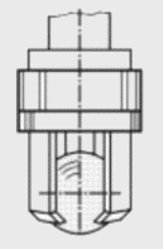
\includegraphics[width=.5\textwidth]{Apendices/Figuras/g1_gray_bg.pdf}
         \caption{Pure enclosing without clamping.}
         \label{fig:g1}
     \end{subfigure}
     \qquad
     \begin{subfigure}[c]{0.25\textwidth}
         \centering
         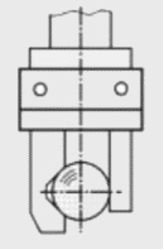
\includegraphics[width=.5\textwidth]{Apendices/Figuras/g2_gray_bg.pdf}
         \caption{Partial form fit combined with clamping force.}
         \label{fig:g2}
     \end{subfigure}
     \qquad
     \begin{subfigure}[c]{0.25\textwidth}
         \centering
         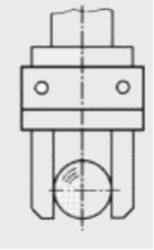
\includegraphics[width=.5\textwidth]{Apendices/Figuras/g3_gray_bg.pdf}
         \caption{Pure force closure.}
         \label{fig:g3}
     \end{subfigure}
	\qquad
     \begin{subfigure}[c]{0.25\textwidth}
         \centering
         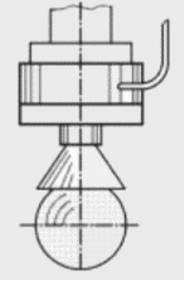
\includegraphics[width=.5\textwidth]{Apendices/Figuras/g4_gray_bg.pdf}
         \caption{Holding with vacuum air (pneumatic force closure).}
         \label{fig:g4}
     \end{subfigure}
     \qquad
     \begin{subfigure}[c]{0.25\textwidth}
         \centering
         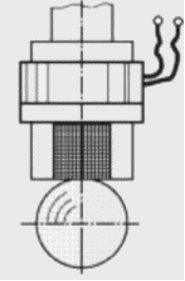
\includegraphics[width=.5\textwidth]{Apendices/Figuras/g5_gray_bg.pdf}
         \caption{Retention using magnetic field (force field).}
         \label{fig:g5}
     \end{subfigure}
     \qquad
     \begin{subfigure}[c]{0.25\textwidth}
         \centering
         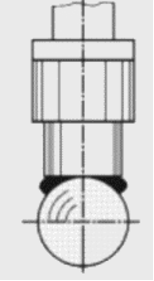
\includegraphics[width=.5\textwidth]{Apendices/Figuras/g6_gray_bg.pdf}
         \caption{Retention using adhesive media.}
         \label{fig:g6}
     \end{subfigure}
    \end{tcolorbox}
    \caption{Forms of grippers according to \cite{monkman2007robot}}
    \label{fig:most_usual_gripper_forms}
  }%end of resize box      
\end{figure}

The use of automatic tool change devices is an option to improve the flexibility, and
applicability of the grippers over the wide variety of objects and workpieces. Besides that, the use of handling machines or dual-arm robots in the automatic process is also a valid alternative (Figure~\ref{fig:alternatives}). Both solutions increase the complexity of the system, and the grasp estimation evaluation may determine which tool is best to complete the task to each object to grasp.

\begin{figure}[h!]
\resizebox{0.75\textwidth}{!}{%
\begin{tcolorbox}
    \centering
    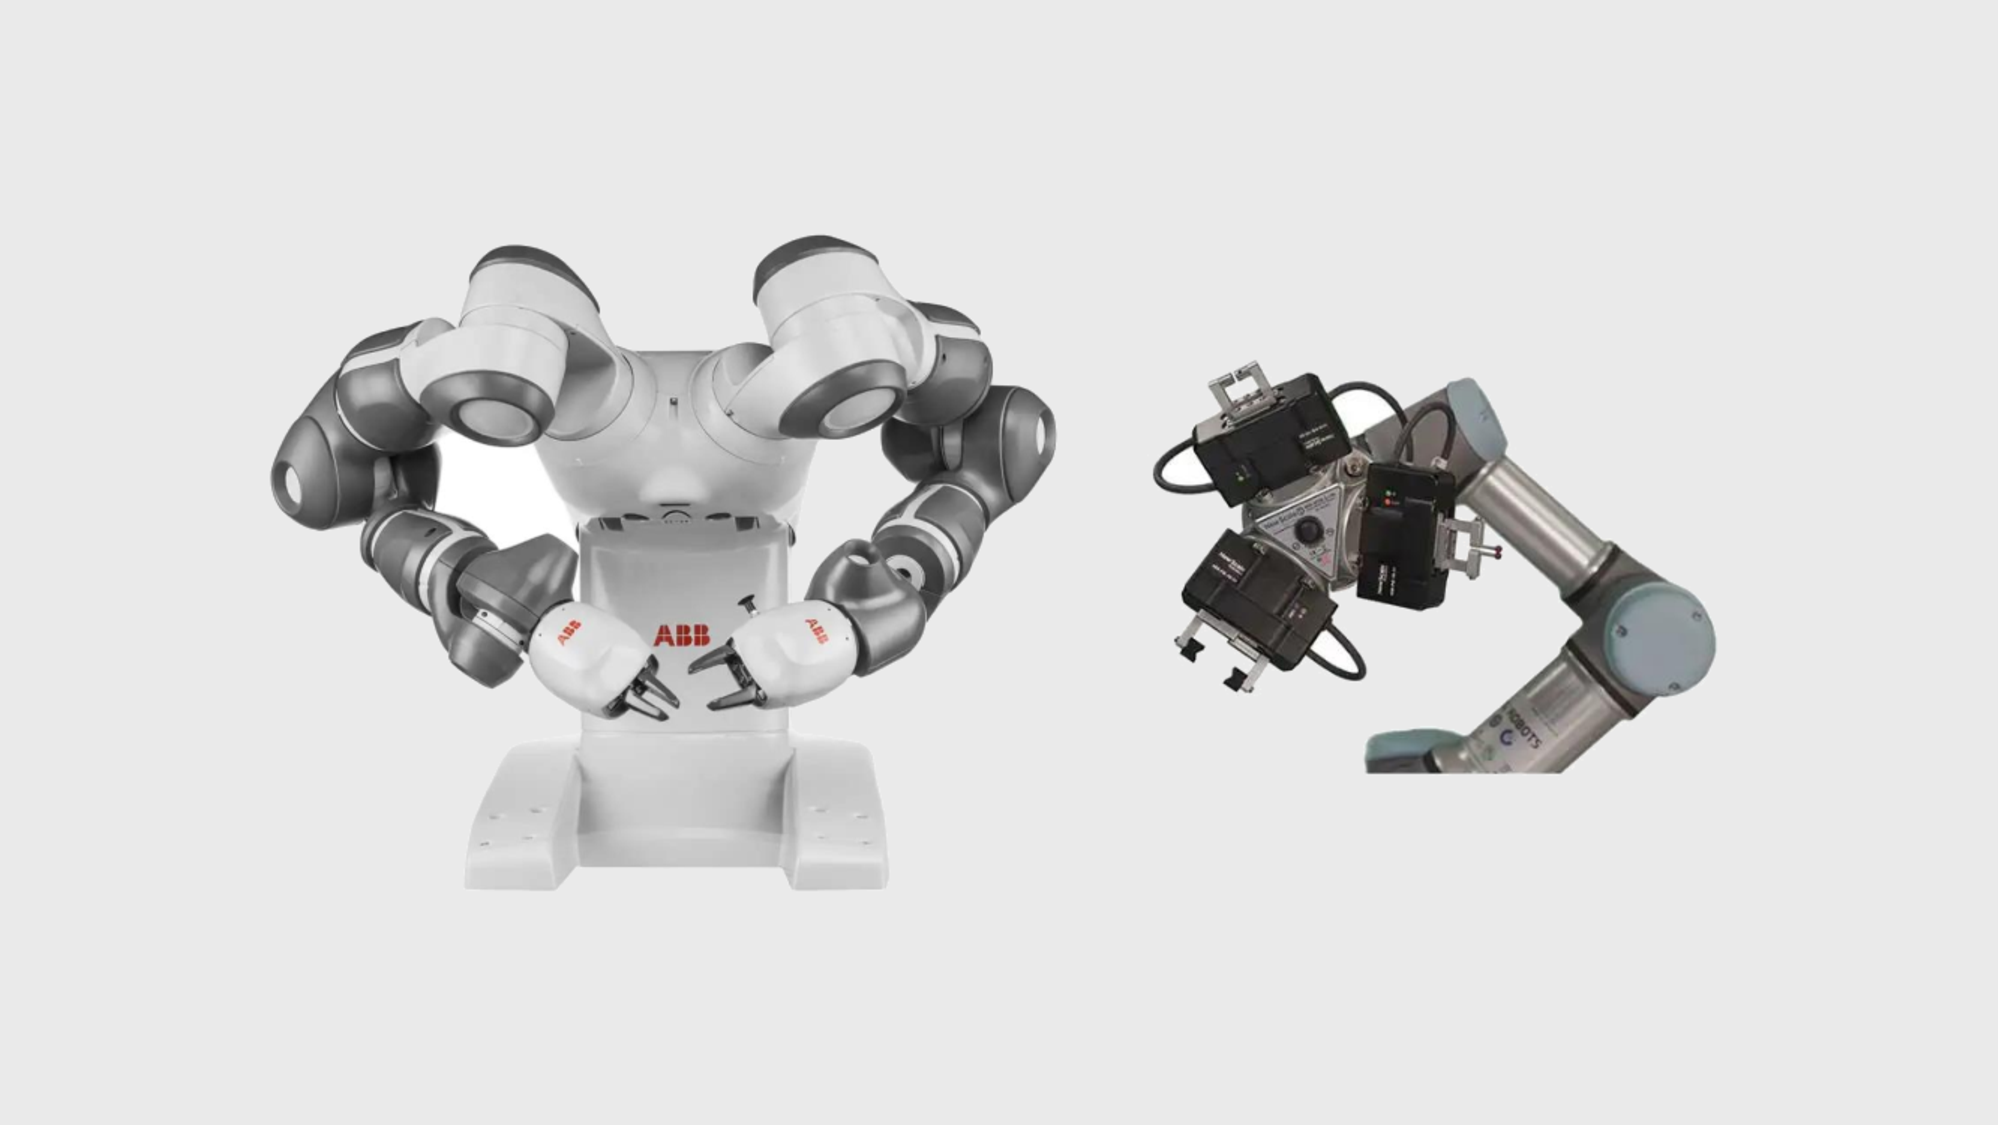
\includegraphics[trim={4cm 3cm 4cm 3cm},clip,width=1\linewidth,angle=0]{Apendices/Figuras/multi_end_effectors_gray_bg.pdf}
\end{tcolorbox}
    \caption{(left) Multi-arm robot~\cite{abb_dual_arm}. (right) Multi-gripper end-effector~\cite{multi_gripper_nsr}}
    \label{fig:alternatives}
}%end resize box
\end{figure}